% !TEX root = task-22.tex
% EGE 2027, task 22. Source IDs and URLs are kept in comments.
% Editable task bank. Append new BankTask blocks at the end of the document.
\documentclass[12pt,a4paper]{article}
\usepackage{physics-textbook}
\usepackage{graphicx,needspace}
\usetikzlibrary{decorations.pathmorphing}
\newif\ifShowSolutions
\ifdefined\TutorEdition
  \ShowSolutionstrue
\else
  \ShowSolutionsfalse % Change to \ShowSolutionstrue to display solutions.
\fi
\newcounter{banktask}
\newsavebox{\BankTaskBox}
\newcommand{\BankTaskContent}[3]{%
  \noindent\textbf{\thebanktask.}\quad #2\par
  \ifShowSolutions
    \Needspace{50mm}% Keep the solution heading with its opening text or diagram.
    #3\par
    \ifdefined\TutorEdition
      \ifcsname TutorSource#1\endcsname
        \nopagebreak\smallskip{\small\csname TutorSource#1\endcsname\par}%
      \fi
    \fi
  \fi
}
\newcommand{\BankTask}[3]{%
  \refstepcounter{banktask}\par\medskip
  \sbox{\BankTaskBox}{\begin{minipage}{\linewidth}%
    \BankTaskContent{#1}{#2}{#3}\end{minipage}}%
  \ifdim\dimexpr\ht\BankTaskBox+\dp\BankTaskBox\relax>\dimexpr\textheight-20mm\relax
    \Needspace{35mm}\BankTaskContent{#1}{#2}{#3}%
  \else
    \Needspace{\dimexpr\ht\BankTaskBox+\dp\BankTaskBox\relax}%
    \noindent\usebox{\BankTaskBox}\par
  \fi
  \medskip
}
\begin{document}


% Source 46782: https://phys-ege.sdamgia.ru/problem?id=46782
\BankTask{46782}{
Камень, поднятый над поверхностью земли, падает без начальной скорости вертикально вниз и за последнюю секунду своего движения проходит путь $\Delta h=10\,\text{м}$. Определите среднюю скорость камня за всё время падения. Сопротивлением воздуха пренебречь.
}{
\smallskip\noindent\textbf{Решение}\par
Средняя скорость камня равна отношению высоты H, с которой бросили камень, к времени его падения $t_0$ до поверхности земли: $v_{\text{ср}} = \frac{H}{t_0} .$
Камень движется вертикально вниз равноускоренно с ускорением свободного падения, следовательно: $H = \frac{g t_0 ^2}{2} ,$ откуда $v_{\text{ср}} = \frac{g t_0}{2} .$ 
Найдём путь $\Delta h,$ пройденный камнем за последнюю секунду падения: 

\[\Delta h = H - h = \frac{g t_0 ^2}{2} - \frac{g ( t_0 - \Delta t ) ^2}{2} ,\]

где $\Delta t = 1 \,\text{с}$ — время, за которое камень прошел путь $\Delta h.$ Отсюда получим: 

$t_0 = \frac{2 \Delta h + g \Delta t ^2}{2 g \Delta t} = \frac{2 \cdot 10 + 10 \cdot 1 ^2}{2 \cdot 10 \cdot 1} = 1{,}5 \,\text{с},$ 
$v_{\text{ср}} = \frac{g t_0}{2} = \frac{10 \cdot 1{,}5}{2} = 7{,}5 \,\text{м/с}.$

Ответ: $v _{\,\text{ср}} = 7{,}5 \,\text{м/с}.$
}

% Source 25400: https://phys-ege.sdamgia.ru/problem?id=25400
\BankTask{25400}{
В процессе прямолинейного равноускоренного движения тело за $2$ секунды прошло путь $20\,\text{м}$, при этом его скорость уменьшилась в $3$ раза. Какой была начальная скорость тела?
}{
\smallskip\noindent\textbf{Решение}\par
\begin{center}\begin{tikzpicture}[x=.65cm,y=.65cm,>=stealth]
\draw[step=1,gray!50,very thin] (0,0) grid (8,8);
\fill[orange!65,opacity=.8] (0,0)--(0,6)--(6,2)--(6,0)--cycle;
\draw[thick] (0,6)--(6,2);
\draw[->,thick] (-1,0)--(8,0) node[below right] {$t,\,\text{с}$};
\draw[->,thick] (0,-.9)--(0,8) node[left] {$v,\,\text{м/с}$};
\node[below left] at (0,0) {$0$};
\node[left] at (0,6) {$v_0$};
\node[left] at (0,2) {$v$};
\node[below] at (6,0) {$t$};
\end{tikzpicture}\end{center}
Поскольку тело двигалось прямолинейно, пройденный путь численно равен площади под графиком функции скорости в зависимости от времени. Поскольку тело двигалось равноускоренно, скорость зависела от времени линейно, а потому искомая площадь (см. рис.) является площадью трапеции с основаниями $v_0$ и \ensuremath{\upsilon} и высотой t:

\[s= \frac{v _0 + v}{2} t.\]

Учитывая, что $v = \frac{v _0}{3} ,$ получаем $s= \frac{2 v _0t}{3} ,$ откуда:

\[v _0= \frac{3s}{2t} = \frac{3 \cdot 20}{2 \cdot 2} =15\,\text{м/с}.\]

Ответ: $15\,\text{м/с}$.
}

% Source 41569: https://phys-ege.sdamgia.ru/problem?id=41569
\BankTask{41569}{
Прямолинейно движущийся поезд последние перед остановкой $1200\,\text{м}$ своего пути преодолел за $2$ минуты. Определите скорость поезда за $30\,\text{с}$ до остановки. Ускорение поезда считать постоянным.
}{
\smallskip\noindent\textbf{Решение}\par
Движение поезда равноускоренное. Поэтому пройденный путь $s= v _0t - \frac{at ^2}{2} ,$ где a  — модуль ускорения поезда. Скорость поезда при этом $v = v _0 - at=0,$ откуда находим скорость в начале торможения $v _0=at.$ 
Объединяя формулы, получаем $s= \frac{at ^2}{2} ,$ откуда ускорение поезда $a= \frac{2s}{t ^2} .$
Из формулы $v = v _1 - at_1=0$ находим скорость поезда за $30\,\text{с}$ до остановки:

\[v _1=at_1= \frac{2st_1}{t ^2} = \frac{2 \cdot 1200 \cdot 30}{120 ^2} =5 \,\text{м/с} .\]

Ответ: $5\,\text{м/с}$.
}

% Source 35210: https://phys-ege.sdamgia.ru/problem?id=35210
\BankTask{35210}{
Бегун бежит прямолинейно с постоянной скоростью $4\,\text{м/с}$. В момент, когда бегун поравнялся с неподвижным велосипедистом, велосипедист начинает двигаться в ту же сторону равноускорено с ускорением $1\,\text{м/с}^{2}$. Найти скорость велосипедиста в момент, когда он догонит бегуна.
}{
\smallskip\noindent\textbf{Решение}\par
Будем считать началом отсчета точку, когда бегун поравнялся с неподвижным велосипедистом. Тогда уравнение движения бегуна при равномерном прямолинейном движении имеет вид:

\[x_1= v _1t.\]

Движение велосипедиста  — равноускоренное прямолинейное без начальной скорости  — описывается уравнением:

\[x_2= \frac{at ^2}{2} .\]

В момент встречи их координаты будут одинаковыми $v _1t= \frac{at ^2}{2} .$ Тогда велосипедист догонит бегуна в момент времени: 

\[t= \frac{2 v _1}{a} .\]

Скорость велосипедиста в этот момент времени будет равной:

\[v _2=at=2 v _1=2 \cdot 4=8 \,\text{м/с} .\]

Ответ: $8\,\text{м/с}$.
}

% Source 35155: https://phys-ege.sdamgia.ru/problem?id=35155
\BankTask{35155}{
Поезд отходит от станции и начинает двигаться равноускоренно. На первом километре пути его скорость увеличилась на $10\,\text{м/с}$. Весь его путь составил $4$ км. Найдите время разгона поезда.
}{
\smallskip\noindent\textbf{Решение}\par
Поскольку поезд отходит от станции, то его начальная скорость $v _0=0.$ Значит, к концу прохождения первого участка его скорость равна $v _1=10 \,\text{м/с} .$ Движение поезда равноускоренное. На первом участке пути $s_1= \frac{v _1 ^2}{2a} ,$ откуда $a= \frac{v _1 ^2}{2s_1} .$
Весь путь, пройденный из состояния покоя, $s= \frac{at ^2}{2} .$ Тогда время разгона поезда равно:

\[t= \sqrt{\frac{2s}{a}} = \sqrt{\frac{4ss_1}{v _1 ^2}} = \frac{2}{v _1} \sqrt{ss_1} = \frac{2}{10} \cdot \sqrt{4 \cdot 10 ^3 \cdot 10 ^3} =400\,\text{с}.\]

Ответ: $400\,\text{с}$.
}

% Source 38204: https://phys-ege.sdamgia.ru/problem?id=38204
\BankTask{38204}{
Небольшой камень, брошенный с ровной горизонтальной поверхности Земли под углом $60^\circ$ к горизонту, достиг максимальной высоты, равной $5\,\text{м}$. Сколько времени прошло от момента броска до того момента, когда скорость камня стала горизонтальной? Сопротивлением воздуха пренебречь.
}{
\smallskip\noindent\textbf{Решение}\par
При движении тела, брошенного под углом к горизонту, на него действует только сила тяжести (по условию сопротивлением воздуха пренебречь). Данная сила является причиной ускорения свободного падения, направленного вертикально вниз.
Выберем ось Oy направленную вертикально вверх. Проекция начальной скорости камня на данную ось $v_{0y}= v _0 \sin \alpha ,$ проекция ускорения $g_y= - g.$ Движение по оси Oy равноускоренное. Тогда проекция скорости на эту ось в любой точке траектории равна $v _y= v_{0y} - gt,$  а проекция перемещения:

\[s_y= \frac{v _y ^2 - v_{0y} ^2}{- 2g} .\]

В точке максимального подъема камня его скорость направлена горизонтально, следовательно, $v _y=0.$
Применим формулы для данных условий: 

$0= v _0 \sin \alpha - gt$ и $H= \frac{v _0 ^2 \sin ^2 \alpha}{2g} .$

При объединении этих формул, получаем:

$v _0 \sin \alpha =gt;$
$H= \frac{gt ^2}{2} .$

Тогда время подъема камня $t= \sqrt{\frac{2H}{g}} .$
При подстановке значений получаем: $t= \sqrt{\frac{2 \cdot 5}{10}} =1\,\text{с}.$

Ответ: $1\,\text{с}$.
}

% Source 25044: https://phys-ege.sdamgia.ru/problem?id=25044
\BankTask{25044}{
Определите скорость, с которой тело было брошено вертикально вниз, если за время падения тела на $15\,\text{м}$ его скорость увеличилась в $2$ раза. Сопротивлением воздуха пренебречь.
}{
\smallskip\noindent\textbf{Решение}\par
Движение тела при отсутствии сопротивления  — равноускоренное с ускорением свободного падения. Тогда $h= \frac{v ^2 - v _0 ^2}{2g} .$ С учетом условия: 

\[h= \frac{4 v _0 ^2 - v _0 ^2}{2g} = \frac{3 v _0 ^2}{2g} .\]

Тогда: 

\[v _0= \sqrt{\frac{2gh}{3}} = \sqrt{\frac{2 \cdot 10 \cdot 15}{3}} =10\,\text{м/с}.\]

Ответ: $10\,\text{м/с}$.
}

% Source 25383: https://phys-ege.sdamgia.ru/problem?id=25383
\BankTask{25383}{
Человек ростом h  =  $1{,}6\,\text{м}$, стоя на земле, кидает мяч из-за головы и хочет перебросить его через забор высотой H  =  $4{,}8\,\text{м}$, находящийся на расстоянии l  =  $6{,}4\,\text{м}$ от него. Определите модуль скорости, с которой необходимо бросить мяч, чтобы он перелетел через забор, коснувшись его в верхней точке своей траектории? Сопротивлением воздуха пренебречь.
}{
\smallskip\noindent\textbf{Решение}\par
Известно, что в верхней точке траектории тела, брошенного под углом к горизонту, скорость направлена горизонтально. Без действия сопротивления воздуха тело движется с ускорением свободного падения. Поэтому по оси Ox движение является равномерным (горизонтальная проекция скорости одинакова на всем пути), по оси Oy движение равноускоренное, при этом в верхней точки траектории вертикальная проекция скорости равна $0$.
Применим закон сохранения энергии для движения мячика от точки броска до верхней точки траектории

\[mgh + \frac{m v _0 ^2}{2} =mgH + \frac{m v _x ^2}{2} .\]

Учитывая, что $v _0 ^2 = v_{0x} ^2 + v_{0y} ^2 ,$ найдем вертикальную проекцию начальной скорости:

\[v_{0y}= \sqrt{2g ( H - h )} = \sqrt{2 \cdot 10 \cdot ( 4{,}8 - 1{,}6 )} =8 \,\text{м/с}.\]

Скорость тела при равноускоренном движении по вертикали равна $v _y= v_{0y} - gt,$ откуда время подъема до верхней точки траектории $t= \frac{v_{0y}}{g} = \frac{8}{10} =0{,}8 \,\text{с}.$
Зная расстояние, которое мяч пролетел по горизонтали, найдем горизонтальную составляющую начальной скорости $v _x= \frac{l}{t} = \frac{6{,}4}{0{,}8} =8 \,\text{м/с}.$
Тогда начальная скорость броска мяча

\[v _0= \sqrt{v_{0x}^2+v_{0y}^2} =8 \sqrt{2} \approx 11{,}3\,\text{м/с}.\]

Ответ: $11{,}3\,\text{м/с}$.
}

% Source 24378: https://phys-ege.sdamgia.ru/problem?id=24378
\BankTask{24378}{
Сталкиваются и слипаются два разных по массе пластилиновых шарика, причем векторы их скоростей непосредственно перед столкновением направлены навстречу друг другу и одинаковы по модулю: $v_1$ = $v_2$  =  $1\,\text{м/с}$. Во сколько раз масса тяжелого шарика больше, чем легкого, если сразу после столкновения их скорость стала равной (по модулю) $0{,}5\,\text{м/с}$?
}{
\smallskip\noindent\textbf{Решение}\par
По закону сохранения импульса для шариков массами m и M при их неупругом взаимодействии $m\vec v _1 + M\vec v _2= ( M + m ) \vec u.$ Учитывая, что скорости шаров до взаимодействия были равными и направлены противоположно, получаем $M v - m v = ( M + m ) u.$ Отсюда $M(v-u)=m(v+u)$. 

\[\frac{M}{m} = \frac{u + v}{v - u} = \frac{0{,}5 + 1}{1 - 0{,}5} =3.\]

Ответ: в $3$ раза.
}

% Source 48533: https://phys-ege.sdamgia.ru/problem?id=48533
\BankTask{48533}{
Тележка массой $200\,\text{кг}$ покоится на земле. В нее запрыгивает мальчик массой $50\,\text{кг}$ со скоростью $4\,\text{м/с}$. Найдите скорость их движения после взаимодействия.
}{
\smallskip\noindent\textbf{Решение}\par
Движение тел поступательное, поэтому тела можно описывать моделью материальной точки. Система отсчета связана с Землей, которую может считать инерциальной системой отсчета. Время взаимодействия мальчика и тележки мало, действием силы трения можно пренебречь. Следовательно, можем применить закон сохранения импульсов тел.
По закону сохранения импульса тел при неупругом взаимодействии $m_1 v = ( m_1 + m_2 ) u,$ откуда находим скорость движения после взаимодействия:

\[u = \frac{m_1 v}{m_1 + m_2} = \frac{50 \cdot 4}{200 + 50} = 0{,}8 \,\text{м/с}.\]

Ответ: $0{,}8\,\text{м/с}$.
}

% Source 741: https://phys-ege.sdamgia.ru/problem?id=741
\BankTask{741}{
\begin{center}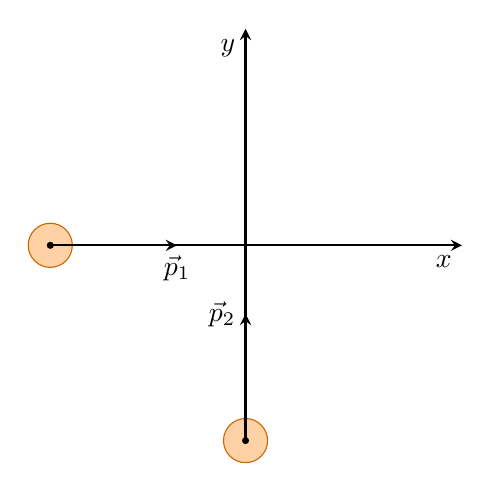
\begin{tikzpicture}[>=stealth]
\draw[->,thick] (-2.67,0)--(2.75,0) node[below left] {$x$};
\draw[->,thick] (0,-2.67)--(0,2.75) node[below left] {$y$};
\filldraw[fill=orange!35,draw=orange!80!black] (-2.48,0) circle (.28) (0,-2.48) circle (.28);
\fill (-2.48,0) circle (.045) (0,-2.48) circle (.045);
\draw[->,thick] (-2.48,0)--(-.87,0) node[below] {$\vec p_1$};
\draw[->,thick] (0,-2.48)--(0,-.87) node[left] {$\vec p_2$};
\end{tikzpicture}\end{center}
По гладкой горизонтальной плоскости по осям x и y движутся две шайбы с импульсами, равными по модулю $p_1=2\,\text{кг} \cdot \,\text{м/с}$ и $p_2=3{,}5\,\text{кг} \cdot \,\text{м/с},$ как показано на рисунке. После соударения вторая шайба продолжает двигаться по оси y в прежнем направлении с импульсом, равным по модулю $p_3=2\,\text{кг} \cdot \,\text{м/с}.$ Найдите модуль импульса первой шайбы после удара.
}{
\smallskip\noindent\textbf{Решение}\par
Поскольку на шайбы не действует никаких внешних сил, для них выполняется закон сохранения импульса:

\[\vec p_1 + \vec p_2=\vec p_3 + \vec p_4.\]

Тогда $\vec p_4=\vec p_1 + \vec p_2 - \vec p_3.$
В проекции на выбранные оси:

$p_{4x}=p_{1x}$
$p_{4y}=p_2 - p_3.$

Тогда модуль вектора импульса первой шайбы после соударения равен

$p_4= \sqrt{p_{4x}^2+p_{4y}^2} = \sqrt{p_1 ^2 + ( p_2 - p_3 ) ^2} =$

$= \sqrt{( 2\,\text{кг} \cdot \,\text{м/с} ) ^2 + ( 3{,}5\,\text{кг} \cdot \,\text{м/с} - 2\,\text{кг} \cdot \,\text{м/с} ) ^2} =2{,}5\,\text{кг} \cdot \,\text{м/с}.$

Ответ: $2{,}5\,\text{кг}$ · м/с.
}

% Source 43099: https://phys-ege.sdamgia.ru/problem?id=43099
\BankTask{43099}{
Мальчик массой $50\,\text{кг}$ находится на тележке массой $50\,\text{кг}$, движущейся по гладкой горизонтальной дороге со скоростью $1\,\text{м/с}$. Каким станет модуль скорости тележки, если мальчик прыгнет с нее со скоростью $2\,\text{м/с}$ относительно дороги в направлении, противоположном первоначальному направлению движения тележки? Ответ запишите в метрах за секунду.
}{
\smallskip\noindent\textbf{Решение}\par
Вдоль горизонтальной оси на тележку и мальчика не действуют силы, поэтому по закону сохранения импульса импульс системы вдоль горизонтальной оси сохраняется:

\[p_0=p_1 + p_2 \Longleftrightarrow ( M + m ) v _0=MV - m v ,\]

где M  — масса тележки, m  — масса мальчика, $v _0$  — проекция начальной скорости тележки, V и $v$  — проекции скоростей тележки и мальчика относительно дороги после прыжка мальчика соответственно.

Найдем проекцию скорости тележки $V:$

\[V= \frac{( M + m ) v _0 + m v}{M} \Longleftrightarrow V= \frac{100\,\text{кг} \cdot 1\,\text{м/с} + 50\,\text{кг} \cdot 2\,\text{м/с}}{50\,\text{кг}} =4\,\text{м/с} .\]

Ответ:  $4\,\text{м/с}$.
}

% Source 38974: https://phys-ege.sdamgia.ru/problem?id=38974
\BankTask{38974}{
Деревянный шар привязан нитью ко дну цилиндрического сосуда с площадью дна S  =  $200\,\text{см}^{2}$. В сосуд наливают воду так, что шар полностью погружается в жидкость, при этом нить натягивается и действует на шар с силой T. Если нить перерезать, то шар всплывёт, а уровень воды изменится на h  =  $5\,\text{см}$. Найдите силу натяжения нити T.
}{
\smallskip\noindent\textbf{Решение}\par
В первом случае на шар действуют сила натяжения нити T и сила тяжести mg, направленные вертикально вниз, сила Архимеда $F_{A1},$ направленная вертикально вверх. Во втором случае на него действуют сила тяжести и сила Архимеда $F_{A2}$ при частичном погружении шара. Запишем второй закон Ньютона для каждого случая при ускорении, равном $0$:

$F_{A1} - mg - T=0,$
$F_{A2} - mg=0.$

В первом случае шар погружен полностью в воду, поэтому $F_{A1}=\rho gV,$ где V  — объем шара. Во втором случае шар погружен частично, поэтому $F_{A2}=\rho gV_{\,\text{пчт}},$ где V$_{\,\text{пчт}}$  — объем погруженной части шара.
Так как по закону Архимеда объем вытесненной жидкости равен объему погруженной части тела, то при его изменении меняется объем жидкости в сосуде на величину $\Delta V=V - V_{\,\text{пчт}}.$
Если обозначить h$_{1}$  — уровень воды в сосуде в первом случае, h$_{2}$  — уровень воды в сосуде во втором случае, то изменение уровня воды равно $h=h_1 - h_2.$ Тогда объем вытесненной воды при всплывании шара изменился на $\Delta V=Sh.$
Объединяя уравнения, находим силу натяжения нити:

\[T=\rho gSh=10 ^3 \cdot 10 \cdot 200 \cdot 10 ^{ - 4 } \cdot 5 \cdot 10 ^{ - 2 } =10\,\text{Н}.\]

Ответ: $T=10\,\text{Н}.$
}

% Source 29874: https://phys-ege.sdamgia.ru/problem?id=29874
\BankTask{29874}{
Однородный деревянный шар массой $m=1{,}6$ кг лежит в сосуде с водой, касаясь дна и не касаясь стенок сосуда, так, что половина шара находится в воде. Определите плотность дерева, если шар  давит на дно с силой $F=6$ Н. Сделайте рисунок с указанием сил, действующих на шар.
}{
\smallskip\noindent\textbf{Решение}\par
\begin{center}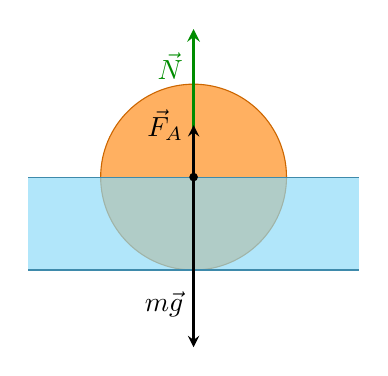
\begin{tikzpicture}[>=stealth]
\filldraw[fill=orange!62,draw=orange!80!black] (0,0) circle (1.18);
\fill[cyan!45,opacity=.68] (-2.1,-1.18) rectangle (2.1,0);
\draw[cyan!65!black] (-2.1,0)--(2.1,0) (-2.1,-1.18)--(2.1,-1.18);
\fill (0,0) circle (.055);
\draw[->,line width=1pt,green!55!black] (0,0)--(0,1.88) node[left,near end] {$\vec N$};
\draw[->,thick] (0,0)--(0,.66) node[left] {$\vec F_A$};
\draw[->,thick] (0,0)--(0,-2.16) node[left,near end] {$m\vec g$};
\end{tikzpicture}\end{center}
 Сила, с которой шар давит на дно, равна по модулю силе реакции опоры по третьему закону Ньютона $F=N.$ Изобразим силы, действующие на деревянный шар (см. рис). 
Шар находится в равновесии, следовательно, $N + F_A=m g.$ Сила Архимеда при погружении шара наполовину, $F_A=\rho_0 g \frac{V}{2} .$ Объем шара $V= \frac{m}{\rho} .$ Объединив формулы, находим плотность дерева, из которого изготовлен шар: 

\[\rho= \frac{\rho_0 g m}{2 \cdot ( m g - N )} = \frac{10 ^3 \cdot 10 \cdot 1{,}6}{2 \cdot ( 1{,}6 \cdot 10 - 6 )} =800 \frac{\,\text{кг}}{\,\text{м} ^3} .\]

Ответ: $800\,\text{кг/м}^{3}$.
}

% Source 29999: https://phys-ege.sdamgia.ru/problem?id=29999
\BankTask{29999}{
Плоская льдина плавает в воде, выступая над ее поверхностью на h  =  $0{,}04\,\text{м}$. Определите массу льдины, если площадь ее поверхности S  =  $2500\,\text{см}^{2}$. Плотность льда равна $900\,\text{кг/м}^{3}$.
}{
\smallskip\noindent\textbf{Решение}\par
\begin{center}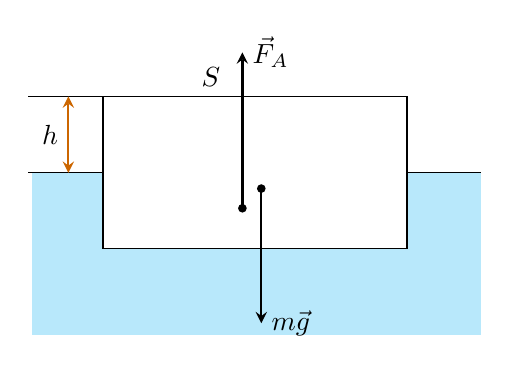
\begin{tikzpicture}[>=stealth]
\fill[cyan!28] (-.9,-1.1) rectangle (4.8,.96);
\filldraw[fill=white,draw=black] (0,0) rectangle (3.86,1.93);
\draw (-.95,1.93)--(0,1.93) (-.95,.96)--(0,.96) (3.86,.96)--(4.8,.96);
\draw[<->,orange!80!black,thick] (-.44,.96)--(-.44,1.93) node[midway,left,black] {$h$};
\node[above] at (1.37,1.93) {$S$};
\fill (1.77,.51) circle (.055) (2.01,.76) circle (.055);
\draw[->,thick] (1.77,.51)--(1.77,2.49) node[right] {$\vec F_A$};
\draw[->,thick] (2.01,.76)--(2.01,-.95) node[right] {$m\vec g$};
\end{tikzpicture}\end{center}
На льдину действуют сила тяжести mg и сила Архимеда $F_A=\rho_{\,\text{в}}gV_{\,\text{пчт}},$ где масса льдины $m=\rho_{\,\text{л}}V,$ объем льдины $V=SH,$ объем погруженной части льдины $V_{\,\text{пчт}}=S ( H - h ) .$
Так как льдина плавает,  то выполняется условие равновесия:

$F_A=m g,$ то есть $\rho_{\,\text{в}} g ( H - h ) S=\rho_{\,\text{л}} g H S,$

 где \ensuremath{\rho}$_{\,\text{в}}$  — плотность воды,  H  — толщина льдины, откуда $H= \frac{\rho_{\,\text{в}} h}{\rho_{\,\text{в}} - \rho_{\,\text{л}}} .$   Следовательно, масса льдины равна

\[m=\rho_{\,\text{л}} S H= \frac{\rho_{\,\text{л}} \rho_{\,\text{в}} S h}{\rho_{\,\text{в}} - \rho_{\,\text{л}}} = \frac{1000 \cdot 900 \cdot 2500 \cdot 10 ^{ - 4 } \cdot 0{,}04}{1000 - 900} =90 \,\text{кг}.\]

Ответ: m  =  $90\,\text{кг}$.
}

% Source 50850: https://phys-ege.sdamgia.ru/problem?id=50850
\BankTask{50850}{
\begin{center}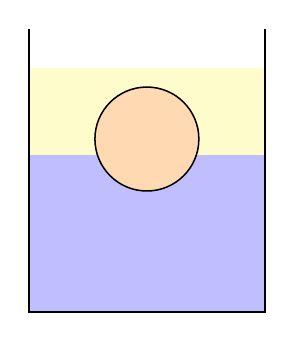
\begin{tikzpicture}[>=stealth,line width=.55pt]\fill[blue!25](0,0)rectangle(3,2);\fill[yellow!20](0,2)rectangle(3,3.1);\draw[thick](0,3.6)--(0,0)--(3,0)--(3,3.6);\draw[fill=orange!30](1.5,2.2)circle(.66);\end{tikzpicture}\end{center}В стакан налита вода, а поверх неё  — керосин. Однородный шар плавает, погружённый в обе жидкости. При этом $\frac{1}{6}$ объёма шара находится в воде, а $\frac{5}{6}$ объёма  — в керосине. Найдите плотность материала шара.
}{
\smallskip\noindent\textbf{Решение}\par
На шар действуют три силы: силы Архимеда со стороны керосина и воды, направленные вертикально вверх и сила тяжести, направленная вертикально вниз. Так как шар плавает, то выполняется условие равновесия:

\[F_{A1} + F_{A2}=mg.\]

Сила Архимеда со стороны керосина $F_{A1}= \frac{5}{6} \rho_{\,\text{к}}gV,$ сила Архимеда со стороны воды $F_{A2}= \frac{1}{6} \rho_{\,\text{в}}gV,$ масса тела $m=\rho V,$ где V  — объем тела. При объединении уравнений находим плотность материала шарика:

\[\rho= \frac{5\rho_{\,\text{к}} + \rho_{\,\text{в}}}{6} = \frac{5 \cdot 800 + 1000}{6} \approx 833 \,\text{кг/м} ^3 .\]

Ответ: $\approx 833 \,\text{кг/м} ^3 .$
}

% Source 24607: https://phys-ege.sdamgia.ru/problem?id=24607
\BankTask{24607}{
\begin{center}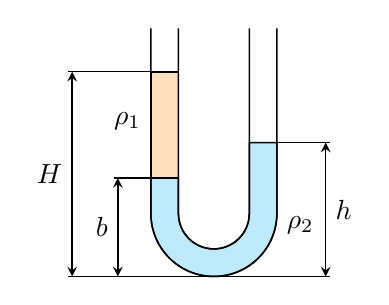
\begin{tikzpicture}[>=stealth,line width=.55pt]\draw[fill=cyan!25](0,1.2)--(0,.75) arc (180:360:.8)--(1.6,1.65)--(1.25,1.65)--(1.25,.75)arc(360:180:.45)--(.35,1.2)--cycle;\draw[fill=orange!25](0,1.2)rectangle(.35,2.55);\draw(0,3.1)--(0,.75)arc(180:360:.8)--(1.6,3.1) (.35,3.1)--(.35,.75)arc(180:360:.45)--(1.25,3.1);\node[left]at(0,1.92){$\rho_1$};\node[right]at(1.6,.6){$\rho_2$};\draw[<->](-1,-.05)--(-1,2.55)node[midway,left]{$H$};\draw[<->](-.42,-.05)--(-.42,1.2)node[midway,left]{$b$};\draw[<->](2.22,-.05)--(2.22,1.65)node[midway,right]{$h$};\draw[thin](-1.05,-.05)--(2.27,-.05) (-1.05,2.55)--(0,2.55) (-.47,1.2)--(0,1.2) (1.6,1.65)--(2.27,1.65);\end{tikzpicture}\end{center}В широкую U-образную трубку с вертикальными прямыми коленами налиты керосин и вода (см. рис.). На рисунке b  =  $10\,\text{см}$, H  =  $30\,\text{см}$. Какова высота жидкости в правом колене?
}{
\smallskip\noindent\textbf{Решение}\par
$1$.  Рассмотрим давление жидкостей в обоих коленах на уровне границы жидкостей. По закону Паскаля давление в обоих коленах на этом уровне должно быть одинаковым.
$2$.  Поскольку высота столба жидкости в левом колене больше, чем в правом, делаем вывод, что в левом колене плотность жидкости меньше, чем в правом, то есть в левом  — керосин, в правом  — вода. Давление жидкости в левом колене равно $p_1=\rho_1g ( H - b ) + p_a,$ в правом колене равно $p_2=\rho_2g ( h - b ) + p_a.$ Из равенства давлений получаем: 

\[h= \frac{\rho_1 ( H - b )}{\rho_2} + b= \frac{800 \cdot ( 30 - 10 )}{1000} + 10=26\,\text{см}.\]

Ответ: $26\,\text{см}$.
}

% Source 35249: https://phys-ege.sdamgia.ru/problem?id=35249
\BankTask{35249}{
Груз массой $200\,\text{г}$ подвешен на пружине жесткостью $100\,\text{Н/м}$ к потолку лифта. Лифт равноускорено движется вниз, набирая скорость. Каково ускорение лифта, если удлинение пружины постоянно и равно $1{,}5\,\text{см}$?
}{
\smallskip\noindent\textbf{Решение}\par
Когда лифт покоился, на груз действовали сила тяжести mg и сила упругости пружины, которая по закону Гука равна $F_{\,\text{упр}}=kx.$ Поскольку груз находился в покое, то выполнялось равенство $mg=kx.$
При движении лифта вниз груз покоится относительно лифта, поэтому по второму закону Ньютона 

$ma=mg - F_{\,\text{упр}};$
$ma=mg - kx.$

Тогда ускорение груза равно:

\[a= g - \frac{kx}{m} = 10 - \frac{100 \cdot 0{,}015}{0{,}2} =2{,}5 \,\text{м/с} ^2 .\]

Ответ: $2{,}5 \,\text{м/с} ^2 .$
}

% Source 43505: https://phys-ege.sdamgia.ru/problem?id=43505
\BankTask{43505}{
\begin{center}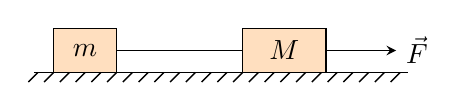
\begin{tikzpicture}[>=stealth,line width=.55pt]\draw[fill=orange!25](0,0)rectangle(.8,.56)node[pos=.5]{$m$};\draw[fill=orange!25](2.4,0)rectangle(3.46,.56)node[pos=.5]{$M$};\draw(.8,.28)--(2.4,.28);\draw[->](3.46,.28)--(4.35,.28)node[right]{$\vec F$};\draw(-.25,0)--(4.5,0);\foreach \x in {-.2,0,...,4.4}{\draw(\x,0)--++(-.12,-.12);}\end{tikzpicture}\end{center}По гладкому горизонтальному столу двигаются два бруска, связанные нерастяжимой и невесомой нитью, которая натянута с силой T  =  $3$ Н. В движение их приводит горизонтально направленная сила F  =  $9$ Н, приложенная к одному из брусков (см. рис.). Чему равна масса M бруска, к которому приложена сила, если масса второго бруска m  =  $0{,}1\,\text{кг}$?
}{
\smallskip\noindent\textbf{Решение}\par
\begin{center}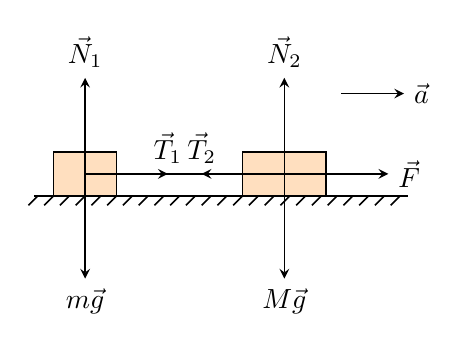
\begin{tikzpicture}[>=stealth,line width=.55pt]\draw[fill=orange!25](0,0)rectangle(.8,.56) (2.4,0)rectangle(3.46,.56);\draw(.8,.28)--(2.4,.28) (-.25,0)--(4.5,0);\foreach \x in {-.2,0,...,4.4}{\draw(\x,0)--++(-.12,-.12);}\draw[->](.4,.28)--(.4,1.5)node[above]{$\vec N_1$};\draw[->](.4,.28)--(.4,-1.05)node[below]{$m\vec g$};\draw[->](.4,.28)--(1.45,.28)node[above]{$\vec T_1$};\draw[->](2.93,.28)--(2.93,1.5)node[above]{$\vec N_2$};\draw[->](2.93,.28)--(2.93,-1.05)node[below]{$M\vec g$};\draw[->](2.93,.28)--(1.88,.28)node[above]{$\vec T_2$};\draw[->](2.93,.28)--(4.25,.28)node[right]{$\vec F$};\draw[->](3.65,1.3)--(4.45,1.3)node[right]{$\vec a$};\end{tikzpicture}\end{center}Изобразим силы, действующие на каждый из брусков. Нить невесома, поэтому силы натяжения $T_1 = T_2 = T.$ Нить нерастяжима, поэтому оба бруска движутся с одинаковым ускорением. Запишем второй закон Ньютона для каждого бруска:

$\overrightarrow{N}_1 + \overrightarrow{T}_1 + m \vec{g} = m \vec{a},$
$\overrightarrow{F} + \overrightarrow{N}_2 + \overrightarrow{T}_2 + M \vec{g} = M \vec{a}.$

 В проекции на горизонтальную ось, сонаправленную с вектором ускорения, получаем:

$F - T = Ma,$
$T = ma.$

 Из этих уравнений находим массу большого бруска:

\[M = \frac{m ( F - T )}{T} = \frac{0{,}1 \cdot ( 9 - 3 )}{3} = 0{,}2 \,\text{кг}.\]

Ответ: $0{,}2\,\text{кг}$.
}

% Source 52049: https://phys-ege.sdamgia.ru/problem?id=52049
\BankTask{52049}{
Небольшой груз массой m  =  $200\,\text{г}$ совершает незатухающие гармонические колебания на невесомой нерастяжимой нити длиной l  =  $2\,\text{м}$. Закон движения этого груза имеет вид: $x ( t ) = 0{,}2 \cos ( \omega t ) ,$ где величина смещения x от положения равновесия измеряется в метрах. Определите максимальную кинетическую энергию груза в процессе колебаний.
}{
\smallskip\noindent\textbf{Решение}\par
Максимальная кинетическая энергия груза равна: 

\[E_k = \frac{m v _{\max} ^2}{2} , \qquad ( 1 )\]

где максимальная скорость груза в процессе колебаний 

\[v _{\max} = \omega A, \qquad ( 2 )\]

а A  — амплитуда колебаний маятника, величину которой можно найти из закона движения: $A = 0{,}2 \,\text{м}.$
Частота \ensuremath{\omega} и период T колебаний маятника связаны соотношением: 

\[\omega = \frac{2 \pi}{T} . \qquad ( 3 )\]

Период колебаний математического маятника можно найти по формуле: 

\[T = 2 \pi \sqrt{\frac{l}{g}} . \qquad ( 4 )\]

Тогда из уравнений ($1$)–($4$) получим: 

\[E_k = \frac{m g A ^2}{2 l} = \frac{0{,}2 \cdot 10 \cdot 0{,}2 ^2}{2 \cdot 2} = 0{,}02 \text \,\text{Дж}.\]

Ответ: $0{,}02\,\text{Дж}$.
}

% Source 51276: https://phys-ege.sdamgia.ru/problem?id=51276
\BankTask{51276}{
\begin{center}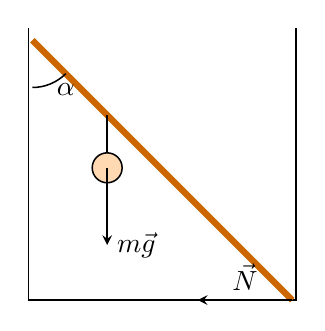
\begin{tikzpicture}[>=stealth,line width=.55pt]\draw(-.05,3.45)--(-.05,0)--(3.35,0)--(3.35,3.45);\draw[orange!80!black,line width=2.3pt](0,3.3)--(3.3,0);\draw(0,2.7)arc(-90:-45:.6)node[below]{$\alpha$};\draw(.95,2.35)--(.95,1.68);\draw[fill=orange!30](.95,1.68)circle(.19);\draw[->](.95,1.68)--(.95,.7)node[right]{$m\vec g$};\draw[->](3.3,0)--(2.1,0)node[midway,above]{$\vec N$};\end{tikzpicture}\end{center}Невесомый стержень длиной $4\,\text{м}$, находящийся в ящике с гладкими дном и стенками, составляет с вертикалью угол $\alpha$  =  $30$° (см. рис.). К стержню на некотором расстоянии от верхнего конца подвешен на нити шар массой $2\,\text{кг}$. Модуль силы нормальной реакции правой стенки ящика, действующей на нижний конец стержня, равен N  =  $7{,}5$ Н. На каком расстоянии x от верхнего конца стержня подвешен шар?
}{
\smallskip\noindent\textbf{Решение}\par
\begin{center}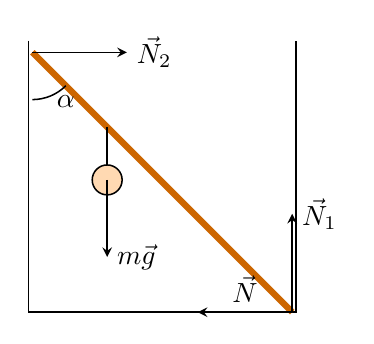
\begin{tikzpicture}[>=stealth,line width=.55pt]\draw(-.05,3.45)--(-.05,0)--(3.35,0)--(3.35,3.45);\draw[orange!80!black,line width=2.3pt](0,3.3)--(3.3,0);\draw(0,2.7)arc(-90:-45:.6)node[below]{$\alpha$};\draw(.95,2.35)--(.95,1.68);\draw[fill=orange!30](.95,1.68)circle(.19);\draw[->](.95,1.68)--(.95,.7)node[right]{$m\vec g$};\draw[->](3.3,0)--(2.1,0)node[midway,above]{$\vec N$};\draw[->](0,3.3)--(1.2,3.3)node[right]{$\vec N_2$};\draw[->](3.3,0)--(3.3,1.25)node[right]{$\vec N_1$};\end{tikzpicture}\end{center}Изобразим силы, действующие на стержень. Для абсолютно твердого тела, каким можно считать стержень, можно применить два условия равновесия:

\[\overrightarrow{N}_2 + \overrightarrow{N}_1 + \overrightarrow{N} + m \vec{g} = 0,\]

где $\overrightarrow{N}_2$  — реакция левой стенки, действующая на верхний конец, $\overrightarrow{N}_1$  —  реакция дна, действующая на верхний конец, $\overrightarrow{N}$  — реакция правой стенки. 
В проекции на горизонтальную ось:

$N_2 - N = 0,$
то есть
$N_2=N.$

Применим правило моментов сил относительно оси, проходящей через нижнюю точку стержня в точке её касания стенки:

\[mg \cdot ( L - x ) \sin \alpha - N_2 L \cos \alpha = 0.\]

Тогда искомое расстояние:

\[x = ( 1 - \frac{N}{mg \cdot \tan \alpha} ) \cdot L = 4 \,\text{м} \cdot ( 1 - \frac{7{,}5 \,\text{Н}}{2 \,\text{кг} \cdot 10 \,\text{м/с} ^2 \cdot \tfrac{1}{\sqrt{3}}} ) = 1{,}4 \,\text{м}.\]

Ответ: $1{,}4\,\text{м}$.
}

% Source 26733: https://phys-ege.sdamgia.ru/problem?id=26733
\BankTask{26733}{
\begin{center}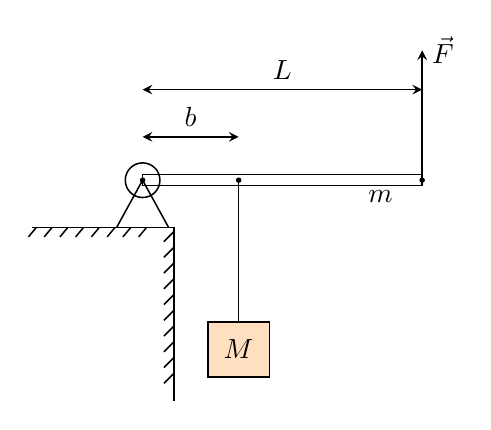
\begin{tikzpicture}[>=stealth,line width=.55pt]\draw(-1.4,-.6)--(.4,-.6)--(.4,-2.8);\foreach \x in {-1.35,-1.15,...,.25}{\draw(\x,-.6)--++(-.1,-.12);}\foreach \y in {-.65,-.85,...,-2.65}{\draw(.4,\y)--++(-.13,-.13);}\draw(-.33,-.6)--(0,0)--(.33,-.6);\draw(0,0)circle(.22);\draw(0,-.07)rectangle(3.55,.07);\fill (0,0)circle(.035) (1.22,0)circle(.035) (3.55,0)circle(.035);\draw[<->](0,1.15)--(3.55,1.15)node[midway,above]{$L$};\draw[<->](0,.55)--(1.22,.55)node[midway,above]{$b$};\draw[->](3.55,0)--(3.55,1.65)node[right]{$\vec F$};\draw(1.22,0)--(1.22,-1.8);\draw[fill=orange!25](.83,-2.5)rectangle(1.61,-1.8)node[pos=.5]{$M$};\node[below]at(3.02,0){$m$};\end{tikzpicture}\end{center}Груз массой M  =  $75\,\text{кг}$ медленно поднимают с помощью рычага, приложив вертикальную силу $\vec F$ (см. рис.). Рычаг, сделанный из однородного стержня массой m  =  $10\,\text{кг}$ и длиной L  =  $4\,\text{м}$, шарнирно закреплен. Определите модуль силы $\vec F,$ если расстояние b от оси шарнира до точки подвеса груза равно $1{,}6\,\text{м}$. Считать, что трение в шарнире отсутствует.
}{
\smallskip\noindent\textbf{Решение}\par
\begin{center}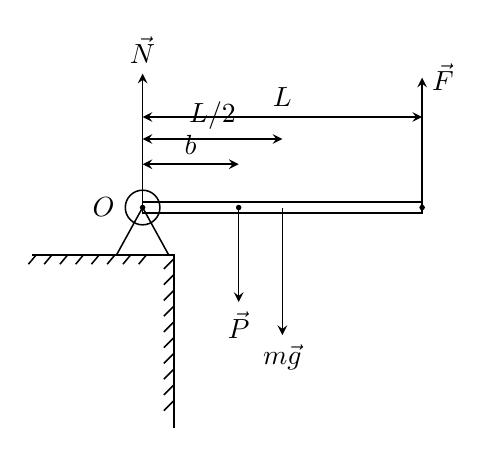
\begin{tikzpicture}[>=stealth,line width=.55pt]\draw(-1.4,-.6)--(.4,-.6)--(.4,-2.8);\foreach \x in {-1.35,-1.15,...,.25}{\draw(\x,-.6)--++(-.1,-.12);}\foreach \y in {-.65,-.85,...,-2.65}{\draw(.4,\y)--++(-.13,-.13);}\draw(-.33,-.6)--(0,0)--(.33,-.6);\draw(0,0)circle(.22);\draw(0,-.07)rectangle(3.55,.07);\fill (0,0)circle(.035) (1.22,0)circle(.035) (3.55,0)circle(.035);\draw[<->](0,1.15)--(3.55,1.15)node[midway,above]{$L$};\draw[<->](0,.55)--(1.22,.55)node[midway,above]{$b$};\draw[->](3.55,0)--(3.55,1.65)node[right]{$\vec F$};\node[left]at(-.23,0){$O$};\draw[->](0,0)--(0,1.7)node[above]{$\vec N$};\draw[<->](0,.87)--(1.775,.87)node[midway,above]{$L/2$};\draw[->](1.22,0)--(1.22,-1.2)node[below]{$\vec P$};\draw[->](1.775,0)--(1.775,-1.62)node[below]{$m\vec g$};\end{tikzpicture}\end{center}$1$.  Рассмотрим силы, действующие на рычаг (см. рис.). 
Считая, что рычаг поднимает груз медленно и равномерно, примем, исходя из третьего и второго законов Ньютона, что $|\vec{P} |=|M \vec{g}|.$
$2$.  Рассмотрим равновесие рычага относительно оси вращения  — шарнира О, указав плечи сил на рисунке. $O: Mg \cdot b + \frac{1}{2} mgL - FL=0.$
Отсюда:

\[F=Mg \cdot \frac{b}{L} + \frac{1}{2} mg=75 \cdot 10 \cdot \frac{1{,}6}{4} + \frac{1}{2} \cdot 10 \cdot 10=350\,\text{Н}.\]

Ответ: F  =  $350$ Н.
}

% Source 25401: https://phys-ege.sdamgia.ru/problem?id=25401
\BankTask{25401}{
Деревянная линейка длиной l  =  $90\,\text{см}$ выдвинута за край стола на $\frac{1}{4}$ часть своей длины. При этом она не опрокидывается, если на ее правом конце лежит груз массой не более $m_1=250\,\text{г}.$ Далее линейку выдвинули вправо за край стола на некоторое расстояние и положили на ее правый конец груз массой $m_2=125\,\text{г}.$ На какое расстояние дополнительно можно выдвинуть линейку во втором опыте, чтобы она не перевернулась?
}{
\smallskip\noindent\textbf{Решение}\par
На линейку в обоих случаях действую сила тяжести линейки, приложенная к ее середине и вес груза. Линейка находится в равновесии, поэтому можно записать правило моментов для каждого случая относительно точки опоры  — края стола. В первом случае плечи силы тяжести линейки и веса груза равны $\frac{l}{4} .$ 
Следовательно, масса линейки равна массе груза $M=m_1=250\,\text{г}.$

\begin{center}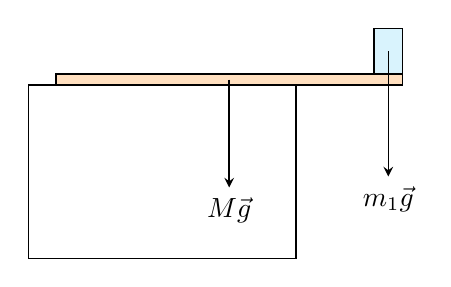
\begin{tikzpicture}[>=stealth,line width=.55pt]\draw(0,-2.2)rectangle(3.4,0);\draw[fill=orange!25](.35,0)rectangle(4.75,.14);\draw[fill=cyan!15](4.39,.14)rectangle(4.75,.72);\draw[->](4.57,.43)--(4.57,-1.16)node[below]{$m_1\vec g$};\draw[->](2.55,.07)--(2.55,-1.3)node[below]{$M\vec g$};\end{tikzpicture}\end{center}

\begin{center}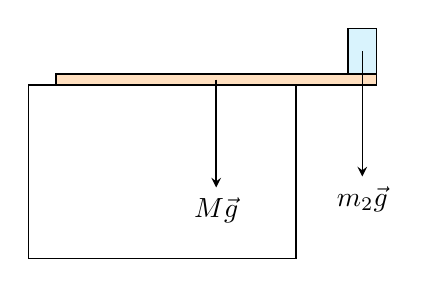
\begin{tikzpicture}[>=stealth,line width=.55pt]\draw(0,-2.2)rectangle(3.4,0);\draw[fill=orange!25](.35,0)rectangle(4.42,.14);\draw[fill=cyan!15](4.06,.14)rectangle(4.42,.72);\draw[->](4.24,.43)--(4.24,-1.16)node[below]{$m_2\vec g$};\draw[->](2.385,.07)--(2.385,-1.3)node[below]{$M\vec g$};\end{tikzpicture}\end{center}

Во втором случае плечо веса груза равно $l_2$ а плечо силы тяжести линейки $\frac{l}{2} - l_2.$
Запишем правило моментов для второго случая:

$m_2gl_2=Mg ( \frac{l}{2} - l_2 ) ,$ откуда плечо веса груза:
$l_2= \frac{Ml}{2 ( m_2 + M )} = \frac{250 \cdot 90}{2 \cdot ( 125 + 250 )} =30\,\text{см}.$

Учитывая, что в первом случае расстояние равнялось $\frac{l}{4} = \frac{90}{4} =22{,}5\,\text{см},$ линейка останется в равновесии, если ее выдвинуть на $7{,}5\,\text{см}$.

Ответ: $7{,}5\,\text{см}$.
}

% Source 29806: https://phys-ege.sdamgia.ru/problem?id=29806
\BankTask{29806}{
\begin{center}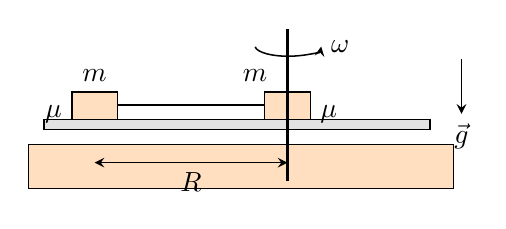
\begin{tikzpicture}[>=stealth,line width=.55pt]\draw[fill=orange!25](-.2,-.75)rectangle(5.2,-.19);\draw[fill=gray!22](0,0)rectangle(4.9,.13);\draw[fill=orange!25](.35,.13)rectangle(.93,.48) (2.8,.13)rectangle(3.38,.48);\draw[thick](3.09,-.65)--(3.09,1.28);\draw(.93,.31)--(2.8,.31);\draw[->](2.68,1.05)arc(185:357:.42 and .13)node[right]{$\omega$};\node[above]at(.64,.48){$m$};\node[above left]at(2.96,.48){$m$};\node[left]at(.35,.19){$\mu$};\node[right]at(3.38,.2){$\mu$};\draw[<->](.64,-.42)--(3.09,-.42)node[midway,below]{$R$};\draw[->](5.3,.9)--(5.3,.2)node[below]{$\vec g$};\end{tikzpicture}\end{center} На горизонтальный диск проигрывателя пластинок положили два одинаковых маленьких грузика массой m каждый, соединенных между собой горизонтальной нитью, один  — в центре, другой  — на расстоянии R  =  $12\,\text{см}$ от оси вращения (см. рисунок). Коэффициенты трения грузиков о диск одинаковы и равны $\mu=0{,}4.$ Диск начали вращать, медленно увеличивая его угловую скорость. При каком значении частоты $v$ вращения грузики свалятся с диска? Считайте, что нить невесома, нерастяжима и вначале не была натянута.
}{
\smallskip\noindent\textbf{Решение}\par
\begin{center}\begin{tikzpicture}[>=stealth,line width=.55pt]\draw[fill=orange!25](-.2,-.75)rectangle(5.2,-.19);\draw[fill=gray!22](0,0)rectangle(4.9,.13);\draw[fill=orange!25](.35,.13)rectangle(.93,.48) (2.8,.13)rectangle(3.38,.48);\draw[thick](3.09,-.65)--(3.09,1.28);\draw(.93,.31)--(2.8,.31);\draw[->](2.68,1.05)arc(185:357:.42 and .13)node[right]{$\omega$};\draw[->](.64,.31)--(.64,1.16)node[above]{$\vec N$};\draw[->](3.09,.31)--(3.09,1.16)node[above]{$\vec N$};\draw[->](.64,.31)--(.64,-.63)node[below]{$m\vec g$};\draw[->](3.09,.31)--(3.09,-.63)node[below]{$m\vec g$};\draw[->](.64,.31)--(1.61,.31)node[above]{$\vec T$};\draw[->](3.09,.31)--(2.12,.31)node[above]{$\vec T$};\draw[->](.64,.13)--(1.57,.13)node[below]{$\vec F_{\text{тр}1}$};\draw[->](3.09,.13)--(4,.13)node[above]{$\vec F_{\text{тр}2}$};\end{tikzpicture}\end{center}$1$.  Проанализируем процессы, происходящие в системе при раскручивании диска проигрывателя, изобразив силы, действующие при этом на грузики (см. рисунок). Силы натяжения, действующие на каждый груз, равны по модулю в силу невесомости нити.
$2$.  До начала раскручивания все тела находятся в покое, и сумма сил, действующих на грузики по вертикали и по горизонтали, равна нулю. Силы нормального давления N грузиков на диск и диска на грузики, одинаковые по третьему закону Ньютона, равны весам грузиков: N  =  mg. Это же соотношение выполняется и после начала раскручивания диска. 
$3$.  После начала медленного раскручивания первый грузик приобретает центростремительное ускорение $a=4 \pi ^2 \nu ^2 R,$ которое возникает по второму закону Ньютона за счет действия силы трения покоя $F_{\,\text{тр}}1 < \,\text{или} \,\text{равно} \mu N=\mu mg,$ откуда $m\omega ^2 R < \,\text{или} \,\text{равно} \mu mg.$
$4$.  В момент достижения предельного значения силы трения покоя первый грузик сдвигается и натягивает нить, то есть появляется сила натяжения нити T, действующая также и на второй грузик и возрастающая по мере ускорения вращения диска. При этом центральный грузик будет оставаться на месте, и $T=F_{\,\text{тр}}2 < \,\text{или} \,\text{равно} \mu N=\mu mg.$
$5$.  Это происходит с ростом $\omega$ до тех пор, пока сила трения $F_{\,\text{тр}}2$ не достигнет своего предельного значения $\mu mg=T_{\,\text{м}},$ после чего второй грузик начнет скользить от оси вращения, и оба грузика свалятся с диска.
$6$.  В момент начала скольжения центрального грузика по диску уравнение движения первого грузика имеет вид: $4 \pi ^2 \nu ^2 Rm=T_{\,\text{м}} + \mu mg=2\mu mg,$ откуда частота вращения диска:

\[\nu = \frac{1}{2 \pi} \sqrt{\frac{2\mu g}{R}} = \frac{1}{2 \cdot 3{,}14} \cdot \sqrt{\frac{2 \cdot 0{,}4 \cdot 10}{0{,}12}} \approx 1{,}3\,\text{Гц}.\]

Ответ: $\approx 1{,}3\,\text{Гц}.$
}

% Source 38971: https://phys-ege.sdamgia.ru/problem?id=38971
\BankTask{38971}{
\begin{center}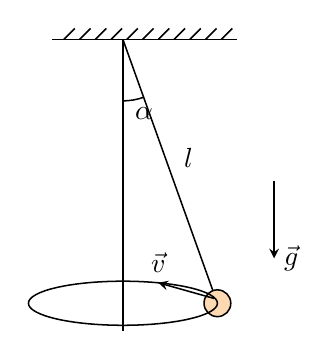
\begin{tikzpicture}[>=stealth,line width=.55pt]\draw(-.9,3.35)--(1.45,3.35);\foreach \x in {-.75,-.55,...,1.25}{\draw(\x,3.35)--++(.14,.14);}\draw(0,3.35)--(0,-.35);\draw(0,3.35)--(1.2,0);\draw(0,2.57)arc(-90:-70:.78)node[below]{$\alpha$};\draw[fill=orange!30](1.2,0)circle(.17);\draw(0,0)ellipse(1.2 and .28);\node[right]at(.65,1.85){$l$};\draw[->](1.16,.06)--(.45,.26)node[above]{$\vec v$};\draw[->](1.92,1.55)--(1.92,.57)node[right]{$\vec g$};\end{tikzpicture}\end{center}Небольшой груз, прикреплённый к нити длиной l  =  $15\,\text{см}$, вращается вокруг вертикальной оси так, что нить отклоняется от вертикали на угол $\alpha$  =  $60$°. С какой скоростью движется груз?
}{
\smallskip\noindent\textbf{Решение}\par
\begin{center}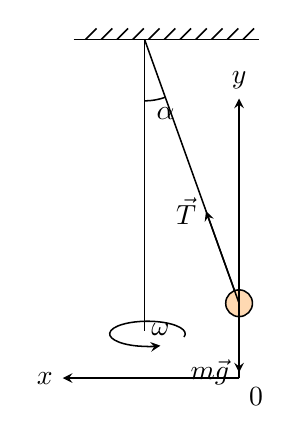
\begin{tikzpicture}[>=stealth,line width=.55pt]\draw(-.9,3.35)--(1.45,3.35);\foreach \x in {-.75,-.55,...,1.25}{\draw(\x,3.35)--++(.14,.14);}\draw(0,3.35)--(0,-.35);\draw(0,3.35)--(1.2,0);\draw(0,2.57)arc(-90:-70:.78)node[below]{$\alpha$};\draw[fill=orange!30](1.2,0)circle(.17);\draw[->](1.2,-.95)--(-1.04,-.95)node[left]{$x$};\draw[->](1.2,-.95)--(1.2,2.6)node[above]{$y$};\node[below right]at(1.2,-.95){$0$};\draw[->](1.2,0)--(.78,1.17)node[left]{$\vec T$};\draw[->](1.2,0)--(1.2,-.88)node[left]{$m\vec g$};\draw[->](.5,-.43)arc(-15:290:.48 and .16)node[above]{$\omega$};\end{tikzpicture}\end{center}Изобразим силы, действующие на грузик. По второму закону Ньютона в ИСО $\overrightarrow{T} + m \vec{g} = m \vec{a},$ где m  — масса грузика, T  — сила натяжения нити. В проекциях на координатные оси получаем:

$Ox: T \sin \alpha = ma,$
$Oy: T \cos \alpha = mg.$

 Следовательно, центростремительное ускорение грузика $a = g \tan \alpha .$ При равномерном движении по окружности со скоростью \ensuremath{\upsilon} по окружности радиусом $R = l \sin \alpha$ грузик имеет центростремительное ускорение $a = \frac{v ^2}{R} .$ Таким образом, скорость, с которой движется грузик, равна

\[v = \sqrt{\frac{gl \sin ^2 \alpha}{\cos \alpha}} = \sqrt{\frac{10 \cdot 0{,}15 \cdot 3}{4 \cdot 0{,}5}} = 1{,}5 \,\text{м/с}.\]

Ответ: $v = 1{,}5 \,\text{м/с}.$
}

% Source 29461: https://phys-ege.sdamgia.ru/problem?id=29461
\BankTask{29461}{
\begin{center}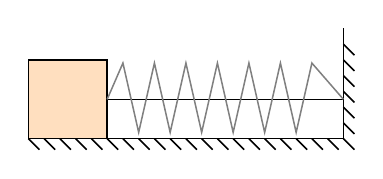
\begin{tikzpicture}[>=stealth,line width=.55pt]\draw[fill=orange!25](0,0)rectangle(1,1);\draw(0,0)--(4,0)--(4,1.4);\draw(1,.5)--(4,.5);\draw[gray](1,.5)--(1.2,.96)\foreach \x in {1.2,1.6,...,3.6}{--(\x+.2,.08)--(\x+.4,.96)}--(4,.5);\foreach \x in {0,.2,...,3.8}{\draw(\x,0)--++(.14,-.14);}\foreach \y in {0,.2,...,1.2}{\draw(4,\y)--++(.14,-.14);}\end{tikzpicture}\end{center}Нить, удерживающая легкую пружину в сжатом состоянии, внезапно оборвалась (см. рисунок). На сколько сантиметров была сжата пружина жесткостью $20\,\text{кН/м}$, если она сообщила бруску массой $20\,\text{г}$ максимальную скорость $10\,\text{м/с}$? Трением бруска о поверхность и массой пружины пренебречь.
}{
\smallskip\noindent\textbf{Решение}\par
В начальном положении в системе пружина обладала потенциальной энергией $E_p= \frac{kx ^2}{2} ,$ брусок находился в покое. Далее брусок приобретет максимальную скорость и кинетическую энергию $E_k= \frac{m v ^2}{2} ,$ когда пружина будет не деформирована. Учитывая, что работа сил тяжести и реакции опоры равна $0$, сила трения отсутствует, применяем закон сохранения энергии $E_p=E_k$ или $\frac{kx ^2}{2} = \frac{m v ^2}{2} .$ Откуда первоначальная деформация пружины: 

\[x= v \sqrt{\frac{m}{k}} =10 \cdot \sqrt{\frac{20\cdot10^{-3}}{20\cdot10^3}} =10 ^{ - 2 } \,\text{м}=1\,\text{см}.\]

Ответ: $1\,\text{см}$.
}

% Source 731: https://phys-ege.sdamgia.ru/problem?id=731
\BankTask{731}{
Подвешенный на нити грузик совершает гармонические колебания. В таблице представлены координаты грузика через одинаковые промежутки времени. Какова примерно максимальная скорость грузика? 

\begin{center}\begin{tabular}{|c|c|c|c|c|c|c|c|c|}\hline
t, c&$0$&$0{,}5$&$1$&$1{,}5$&$2$&$2{,}5$&$3$&$3{,}5$\\\hline
x, см&$6$&$3$&$0$&$3$&$6$&$3$&$0$&$3$\\\hline
\end{tabular}\end{center}
}{
\smallskip\noindent\textbf{Решение}\par
Максимальная скорость груза маятника связана с амплитудой колебаний и циклической частотой соотношением: 

\[v _{\,\text{м}}=x_{\,\text{м}} \omega_0.\]

Из таблицы видно, что при колебаниях смещение меняется от $0$ до $6\,\text{см}$. Следовательно, в положении равновесия смещение равно $3\,\text{см}$, а амплитуда колебаний равна $x_{\,\text{м}}=3\,\text{см},$ период $T=2\,\text{с},$ а значит, циклическая частота:

\[\omega_0= \frac{2 \pi}{T} = \frac{2 \pi}{2\,\text{с}} = \pi \,\text{рад/с}.\]

Таким образом, максимальная скорость груза равна приблизительно:

\[v _{\,\text{м}}=0{,}03\,\text{м} \cdot 3{,}14\,\text{с}^{-1}\approx 0{,}09\,\text{м/с}.\]

Ответ: $0{,}09\,\text{м/с}$.
}

% Source 50844: https://phys-ege.sdamgia.ru/problem?id=50844
\BankTask{50844}{
Груз массой $2\,\text{кг}$, закреплённый на пружине жесткостью $200\,\text{Н/м}$, совершает горизонтальные гармонические колебания. Максимальное ускорение груза при этом равно $10\,\text{м/с}^{2}$. Какова максимальная скорость груза?
}{
\smallskip\noindent\textbf{Решение}\par
При гармонических колебаниях максимальная сила $F_{\max}=kA,$ где A  — амплитуда колебаний. По второму закону Ньютона $F_{\max}=ma_{\max}.$ Тогда амплитуда колебаний равна

\[A = \frac{ma_{\max}}{k} .\]

Для гармонических колебаний выполняется закон сохранения энергии:

\[\frac{kA ^2}{2} = \frac{m v _{\max} ^2}{2} .\]

Объединяя уравнения, находим максимальную скорость груза:

\[v _{\max}=a_{\max} \sqrt{\frac{m}{k}} =10 \cdot \sqrt{\frac{2}{200}} =1 \,\text{м/с}.\]

Ответ: $1\,\text{м/с}$.
}

% Source 32266: https://phys-ege.sdamgia.ru/problem?id=32266
\BankTask{32266}{
\begin{center}\begin{tikzpicture}[>=stealth,line width=.55pt]\draw[->](0,.32)--(0,-6.75)node[below]{$y,\ \text{м}$};\node[left]at(0,.28){$O$};\foreach \i in {0,2,...,60}{\draw(-.09,-\i/10)--(.09,-\i/10);}\foreach \i in {0,10,...,60}{\draw(-.16,-\i/10)--(.16,-\i/10)node[right]{$\i$};}\foreach \i in {0,6,24,54}{\fill[orange!75!black](-.74,-\i/10)circle(.075);}\end{tikzpicture}\end{center}На неизвестной планете, лишенной атмосферы, космонавт уронил предмет, четыре последовательных положения которого через каждую секунду показаны на рисунке. Покажите, что движение предмета равноускоренное, и определите проекцию вектора ускорения, с которым падает предмет, на направление оси y.
}{
\smallskip\noindent\textbf{Решение}\par
Найдем ускорение шарика в моменты времени $t=1, 2, 3 \,\text{с},$ исходя из формулы равноускоренного движения без начальной скорости: $s= \frac{at ^2}{2} ,$ откуда $a= \frac{2s}{t ^2} .$ Получаем:

$a_1= \frac{2 \cdot 6}{1 ^2} =12 \,\text{м/с} ^2 ;$
$a_2= \frac{2 \cdot 24}{2 ^2} =12 \,\text{м/с} ^2 ;$
$a_3= \frac{2 \cdot 54}{3 ^2} =12 \,\text{м/с} ^2 .$

Таким образом, в любые промежутки времени ускорение оставалось неизменным. Следовательно, движение на планете было равноускоренным с ускорением $a=12 \,\text{м/с} ^2 .$

Ответ: движение равноускоренное; ускорение $12\,\text{м/с}^{2}$.
}

% Source 41563: https://phys-ege.sdamgia.ru/problem?id=41563
\BankTask{41563}{
\begin{center}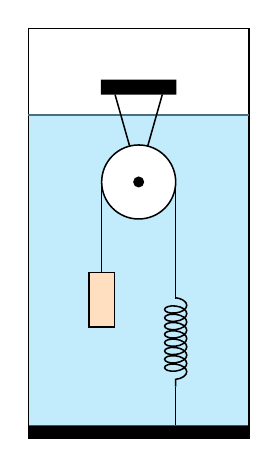
\begin{tikzpicture}[>=stealth,line width=.55pt]\fill[cyan!24](0,0)rectangle(2.8,4.1);\draw(0,0)rectangle(2.8,5.2);\draw[cyan!45!black](0,4.1)--(2.8,4.1);\fill(0,0)rectangle(2.8,.16) (.92,4.36)rectangle(1.88,4.55);\draw(1.1,4.36)--(1.4,3.3)--(1.7,4.36);\draw[fill=white](1.4,3.25)circle(.47);\fill(1.4,3.25)circle(.07);\draw(.93,3.25)--(.93,2.1) (1.87,3.25)--(1.87,1.77);\draw[fill=orange!25](.77,1.41)rectangle(1.09,2.1);\draw[decorate,decoration={coil,segment length=3pt,amplitude=4pt}](1.87,1.78)--(1.87,.65);\draw(1.87,.65)--(1.87,.16);\end{tikzpicture}\end{center}На рисунке представлена система тел, состоящая из неподвижного блока с перекинутой через него лёгкой и нерастяжимой нитью, к концам которой привязаны груз массой m  =  $0{,}8\,\text{кг}$ и объёмом V  =  $100\,\text{см}^{3}$ и лёгкая пружина жёсткостью k  =  $100$ H/м. Эта система находится в покое и  погружена в сосуд с жидкостью плотностью $\rho = 900\,\text{кг/м} ^3 .$ Нижний конец пружины прикреплён к дну сосуда. Как и на сколько изменится сила натяжения нити, действующая на пружину, если сосуд будет заполнен не первоначальной жидкостью, а таким же объёмом воды? Считать, что трение в оси блока отсутствует.
}{
\smallskip\noindent\textbf{Решение}\par
\begin{center}\begin{tikzpicture}[>=stealth,line width=.55pt]\fill[cyan!24](0,0)rectangle(2.8,4.1);\draw(0,0)rectangle(2.8,5.2);\draw[cyan!45!black](0,4.1)--(2.8,4.1);\fill(0,0)rectangle(2.8,.16) (.92,4.36)rectangle(1.88,4.55);\draw(1.1,4.36)--(1.4,3.3)--(1.7,4.36);\draw[fill=white](1.4,3.25)circle(.47);\fill(1.4,3.25)circle(.07);\draw(.93,3.25)--(.93,2.1) (1.87,3.25)--(1.87,1.77);\draw[fill=orange!25](.77,1.41)rectangle(1.09,2.1);\draw[decorate,decoration={coil,segment length=3pt,amplitude=4pt}](1.87,1.78)--(1.87,.65);\draw(1.87,.65)--(1.87,.16);\draw[->](-.25,5.18)--(-.25,.05)node[below]{$y$};\node[left]at(-.25,5.18){$0$};\draw[->](.93,1.77)--(.93,2.93)node[left]{$\vec T_1$};\draw[->](.93,1.77)--(.93,2.55)node[right]{$\vec F_{\text{арх}}$};\draw[->](.93,1.77)--(.93,.83)node[below]{$m\vec g$};\end{tikzpicture}\end{center}Изобразим силы, действующие на груз: сила тяжести $m\vec g,$ сила натяжения нити $\vec T_1,$ сила Архимеда $\vec F_A.$ По третьему закону Ньютона сила натяжения нити равна силе упругости, возникающей в пружине, равна силе натяжения $\vec T_1,$ так как нить легкая и сила трения в блоке отсутствует. В инерциальной системе отсчета, связанной с Землей, условие равновесия груза имеет вид:

\[m\vec g + \vec T_1 + \vec F_A=0.\]

В проекции на ось Oy: $T_1 + F_A - mg=0,$ где сила Архимеда равна $F_A=\rho gV.$ Откуда сила натяжения нити, действующая на груз, погруженный в жидкость, равна

\[T_1=mg - \rho gV.\]

Если  жидкость заменить на воду, то сила натяжения нити станет равной

\[T_2=mg - \rho_{\,\text{в}} gV.\]

Поскольку плотность воды  больше плотности жидкости, то сила Архимеда увеличится, а сила натяжения уменьшится на величину, равную

\[T_1 - T_2=gV ( \rho_{\,\text{в}} - \rho ) =10 \cdot 10 ^{ - 4 } \cdot ( 1000 - 900 ) =0{,}1\,\text{Н}.\]

Ответ: уменьшится на $0{,}1$ Н.
}

\end{document}
